\documentclass[review]{elsarticle}

%\usepackage{lineno}
\usepackage{hyperref}
\usepackage{pdflscape}
%\modulolinenumbers[5]

\journal{Contributions to Mineralogy and Petrology}

%%%%%%%%%%%%%%%%%%%%%%%
%% Elsevier bibliography styles
%%%%%%%%%%%%%%%%%%%%%%%
%% To change the style, put a % in front of the second line of the current style and
%% remove the % from the second line of the style you would like to use.
%%%%%%%%%%%%%%%%%%%%%%%

%% Numbered
%\bibliographystyle{model1-num-names}

%% Numbered without titles
%\bibliographystyle{model1a-num-names}

%% Harvard
\bibliographystyle{model2-names.bst}\biboptions{authoryear}

%% Vancouver numbered
%\usepackage{numcompress}\bibliographystyle{model3-num-names}

%% Vancouver name/year
%\usepackage{numcompress}\bibliographystyle{model4-names}\biboptions{authoryear}

%% APA style
%\bibliographystyle{model5-names}\biboptions{authoryear}

%% AMA style
%\usepackage{numcompress}\bibliographystyle{model6-num-names}

%% `Elsevier LaTeX' style
%\bibliographystyle{elsarticle-num}
%%%%%%%%%%%%%%%%%%%%%%%

\begin{document}

\begin{frontmatter}

\title{Excess thermodynamic and elastic properties of mineral and melt solutions: modelling and implications for phase relations and seismic velocities}
%\tnotetext[mytitlenote]{Fully documented templates are available in the elsarticle package on \href{http://www.ctan.org/tex-archive/macros/latex/contrib/elsarticle}{CTAN}.}

%% Group authors per affiliation:
\author{R. Myhill}
\address{Bayerisches Geoinstitut, Universit\"{a}t Bayreuth, Universit\"{a}tsstrasse 30, 95447 Bayreuth, Germany}
\cortext[mycorrespondingauthor]{Corresponding author: R. Myhill}
\ead{myhill.bob@gmail.com}

\begin{abstract}
Thermodynamic models of solid and liquid solutions are increasingly used to calculate phase relations and seismic properties over large pressure and temperature ranges. Research into mantle phase relations, subduction and differentiation of the early Earth frequently involves calculations spanning thousands of Kelvin and tens of gigapascals. Over such huge ranges, excess entropy and volume are unlikely to remain constant with respect to pressure and temperature. For example, absolute excess volumes usually decrease with increasing pressure. The implication is that to provide a good estimate of phase relations and seismic velocities, solution models must be flexible enough to accommodate changes in elastic and thermodynamic derivatives, such as the bulk modulus.

This paper describes an extension to the subregular Margules mixing model which employs intermediate compounds to define the excess thermodynamic properties of solid solutions. Mathematical derivations are provided for excess thermodynamic properties (enthalpy, entropy, volume) and their pressure and temperature derivatives (bulk modulus, thermal expansion etc.). Heuristics are suggested for intermediate compounds where individual thermodynamic properties are poorly constrained.

Examples of pyroxene, garnet and melt solutions are presented, which show that accurate modelling of phase relations and seismic velocities requires absolute excess volumes to decrease as a function of pressure. The formulation proposed here allows for a wealth of experimental data to be incorporated into solution models, and is expected to be important for geochemical and geophysical models of the Earth and other planetary bodies.
\end{abstract}

\begin{keyword}
high pressure \sep excess properties \sep solution model \sep solid \sep melt \sep elasticity
\end{keyword}

\end{frontmatter}

\linenumbers

\section{Introduction}

Solution models are a vital part of estimating phase relations at high pressure and temperatures. Typically, experimental estimates of excess Gibbs free energy across a binary solution are fit to some functional form (often quadratic, cubic). The variables for these functions are called interaction parameters, and generally have the form
\begin{equation}
  W_{ij}^{\mathcal{G}} = W_{ij}^{\mathcal{H}} + W_{ij}^{\mathcal{V}}P + W_{ij}^{\mathcal{S}}T
  \label{eqn:trad_form}
\end{equation}
\noindent The enthalpic $\mathcal{H}$, entropic $\mathcal{S}$ and volumetric $\mathcal{V}$ contributions to each parameter can be derived from calorimetry, phase relations and X ray diffraction. These models have been extremely successful in describing the thermodynamic properties of solid solutions at crustal pressures and temperatures. Under such conditions, the linear pressure and temperature approximation in Equation \ref{eqn:trad_form} is perfectly reasonable, as deviations from constant volume and entropy excesses are small. However, thermodynamic models are now being extended over much larger pressure and temperature ranges \citep{SLB2011, HP2011, HHPH2013, DKS2013}. It is unlikely that excess properties will remain constant over these ranges. For example, imagine two crystal lattices ($A_xO_y$ and $B_xO_y$) comprising cations with different ionic radii and field strengths. The properties of the cations (and anion) result in different unit cell volumes and compressibilities; typically the lattice with the larger cationic radius will have a large volume and smaller bulk modulus \citep{AA1970}. Now imagine a third lattice with intermediate composition ($[A_{1-z}B_z]_xO_y$). This lattice will typically exhibit distortions which result in a positive or negative excess volume, as a direct result of changing the average cation-anion bond length relative to the sum of the endmembers (Vegard's Law). It is reasonable to suggest that longer bonds will be more compressible, and that therefore a positive excess volume will result in a negative excess bulk modulus. The reverse is also true; shorter bonds are likely to be less compressible. Of course, compression in complex minerals is unlikely to be well-described by a simple isotropic change in bond length. Nevertheless, other compression mechanisms such as polyhedral rotation are likely to be affected in a similar way; in general, a smaller volume will reduce the flexibility of the structure.

Thermoelastic models are also increasingly being used to interpret seismic data in terms of the temperature and composition of the deep Earth. Studies have focussed on Earth's mantle \citep[e.g.][]{DGDSBR2012, MCDRT2012, DCT2012} and core \citep[e.g.][]{SGGFMM2000,SFGMM2004}, and with the successful deployment of seismometers may soon extend to Mars \citep{GLZR2014}. Again, the bulk modulus imposed by the constant excess volume approximation may be a significant and unnecessary contributor to error in these studies, especially for metallic liquids, where excess volumes at low pressures are often very large. 

The current study addresses the problems outlined above by adapting the subregular Margules mixing model, using intermediate compounds to describe the excess properties of the solid solution. The added flexibility comes with a large increase in the number of free parameters, so useful heuristics are also provided to estimate these where independent constraints are unavailable. The new formulation should enable a large number of studies on elastic properties of solid solutions to be incorporated into thermodynamic models. This study also highlights the need for high quality equation of state and seismic velocity data for intermediate compositions within solid solutions.

\section{Theory} 
\subsection{The Extended Subregular Margules (ESM) model}
The subregular Margules mixing model within a binary system $A$-$B$ approximates excess Gibbs free energies at any given pressure and temperature as a cubic function of composition \citep{HW1989}:
\begin{equation}
  \mathcal{G}^{xs} = X_B (1-X_B) \left(W_{AB} X_B + W_{BA} (1-X_B) \right)
  \label{eqn:subreg}
\end{equation}

In the special case that $W_{AB} = W_{BA}$, the function is a quadratic. I can define the Gibbs interaction parameter in terms of the Gibbs free energy of a 50:50 intermediate compound ($AB$) and the endmembers $A$ and $B$:

\begin{equation}
  W^{\mathcal{G}}_{AB} = 4(\mathcal{G}_{AB} + T\mathcal{S}^{\textrm{conf}}_{AB}) - 2(\mathcal{G}_A + \mathcal{G}_B)
\end{equation}
\noindent where $\mathcal{S}^{\textrm{conf}}_{AB}$ is the configurational entropy of the intermediate compound. In the more general case that $W_{AB} \neq W_{BA}$, Equation \ref{eqn:subreg} can be thought of as two symmetric interaction parameters with contributions that depend on the composition. Two intermediate compounds ($AB$ and $BA$) are then required to describe the properties of the solution (Figure \ref{fig:schematic}).

\begin{figure}[ht!]
  \centering
  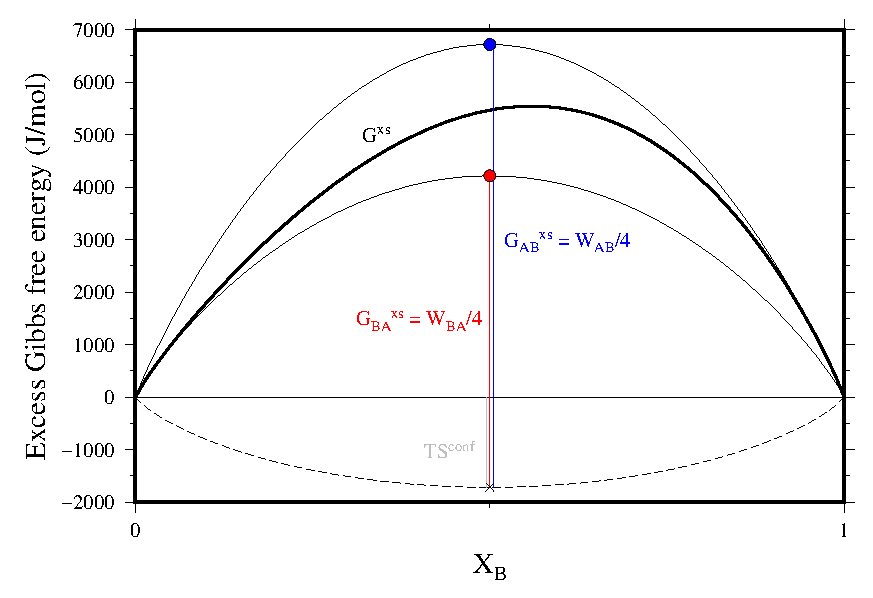
\includegraphics[width=0.8\textwidth]{figures/schematic}
  \caption{Schematic illustration of excess energies within a binary subregular solution model.}
  \label{fig:schematic}
\end{figure}


Expanding the subregular solution model beyond a binary system, the excess nonconfigurational Gibbs free energy is \citep{HW1989} 
\begin{equation}
  \mathcal{G}^{xs} = \sum_{i=1}^n \sum_{j>1}^n X_i X_j \left ( W_{ij} X_j + W_{ji} X_i + 0.5 (W_{ij} + W_{ji}) \sum_k^n (1-\delta_{ik})(1-\delta_{jk}) X_k \right)
  \label{xs}
\end{equation}

Each of the individual $W_{ij}$ terms in Equation \ref{xs} can be determined via the properties of an intermediate compound, just as described in the binary $A$-$B$ system (Equation \ref{eqn:subreg}). The properties of the solid solution with composition $\mathbf{X}$ are then defined as follows:

\begin{eqnarray}
\mathcal{G} = \sum_i X_i \mathcal{G}_i + \mathcal{G}^{xs} \\
\mathcal{H} = \sum_i X_i \mathcal{H}_i + \mathcal{H}^{xs} \\
\mathcal{S} = \sum_i X_i \mathcal{S}_i + \mathcal{S}^{xs} \\
\mathcal{V} = \sum_i X_i \mathcal{V}_i + \mathcal{V}^{xs} \\
C_P = \sum_i X_i C_P  + T \left( \frac{\partial \mathcal{S}}{\partial T} \right)_P^{xs} \\
\alpha = \frac{1}{\mathcal{V}} \left ( \sum_i X_i \alpha_i \mathcal{V}_i + \left( \frac{\partial \mathcal{V}}{\partial T} \right)_P^{xs} \right) \label{alpha} \\
K_T = \frac{\mathcal{V}}{\sum_i \frac{X_i \mathcal{V}_i }{K_{Ti}} - \left( \frac{\partial \mathcal{V}}{\partial P} \right)_T^{xs} } \label{K_T} \\
C_V = C_P - \mathcal{V} T \alpha^2 K_T \\
K_S = K_T \frac{C_P}{C_V} \\
\gamma = \frac{\alpha K_T \mathcal{V}}{C_V}   
\end{eqnarray}

With the exception of the enthalpy excess, excess terms ($\mathcal{S}^{xs}$, $\mathcal{V}^{xs}$ etc) are derived in the same way as the excess Gibbs free energy (Equation \ref{xs}), with interaction terms defined as follows:

\begin{eqnarray}
  W^{\mathcal{S}}_{ij} = 4 (\mathcal{S}_{ij} - \mathcal{S}^{\textrm{conf}}_{ij}) - 2(\mathcal{S}_i + \mathcal{S}_j) \\
  W^{\mathcal{V}}_{ij} = 4 \mathcal{V}_{ij} - 2(\mathcal{V}_i + \mathcal{V}_j) \\
  W^{\partial\mathcal{V}/\partial P}_{ij} = -4 \mathcal{V}_{ij}/K_{T{ij}} + 2(\mathcal{V}_{i}/K_{T{i}} + \mathcal{V}_{j}/K_{T{j}}) \\
  W^{\partial\mathcal{V}/\partial T}_{ij} = 4 \alpha_{ij} \mathcal{V}_{ij} - 2(\alpha_{i} \mathcal{V}_i + \alpha_{j} \mathcal{V}_j) \\
  W^{\partial\mathcal{S}/\partial T}_{ij} = \frac{4 C_{P{ij}} - 2(C_{P{i}} + C_{P{j}})}{T} 
\end{eqnarray}

Finally, excess enthalpy is defined as
\begin{equation}
 \mathcal{H}^{xs} = \mathcal{G}^{xs} + T\mathcal{S}^{xs}
\end{equation}

\subsection{Heuristics}
It is often the case that endmembers are particularly well studied, while the properties of the solid solution are constrained only by enthalpies of solution and volumes at room temperature and pressure. The remaining properties of the intermediate compounds must be estimated by the user. In this study, we suggest that the following heuristics be used:
\begin{eqnarray}
  \mathcal{S}_{ij} = 0.5(\mathcal{S}_i + \mathcal{S}_j) + \mathcal{S}^{\textrm{conf}}_{ij} \\
  C_{P{ij}} = 0.5(C_{P{i}} + C_{P{j}}) \\
  \alpha_{ij} = 0.5 \mathcal{V} \left(\frac{\alpha_i}{\mathcal{V}_i} + \frac{\alpha_j}{\mathcal{V}_j}\right)\\
  K'_{T} = -\frac{\partial}{\partial P} \left (\mathcal{V}\left( \frac{\partial P}{\partial \mathcal{V}} \right)_T \right) \sim \mathcal{V} \left(\sum_i \frac{X_i \mathcal{V}_i}{K'_{Ti} + 1} \right)^{-1} - 1
\end{eqnarray}

If excess volumes are zero, it is likely that they will remain zero as temperatures and pressures increase. In this case, the bulk modulus is given by Equation \ref{K_T}, with the differential term equal to zero. In contrast, non-zero excess volumes are unlikely to remain constant with pressure and temperature. I suggest that, in the absence of other data a useful heuristic is $\left( \frac{\partial \mathcal{V}}{\partial P} \right)_T^{xs} \rightarrow 0$ as $P \rightarrow \infty$.

A useful way to view the change in bulk modulus across a solid solution is to compare the excess bulk modulus to that implied by the $K_TV =$ \emph{constant} rule of thumb proposed by \cite{AA1970} to estimate the compressibility of endmembers based on their molar volumes. The heuristic we propose in this study predicts a larger excess term than that suggested by the rule of thumb, which we describe using a factor $\xi$:

\begin{equation}
  K_{T} \sim 0.5(K_{Ti} + K_{Tj}) + \xi \left(\frac{K_{Ti}\mathcal{V}_{j} + K_{Tj}\mathcal{V}_{j}}{2 \mathcal{V}} - 0.5(K_{Ti} + K_{Tj})\right)
  \label{K_T_heuristic}
\end{equation}
\noindent Typically, a value of $\sim$6 provides a useful estimate of $\xi$.

Now that we have described the new model and heuristics related to the construction of intermediate compounds, we turn to a few geologically relevant examples. The models in this study are all implemented in the open software \emph{burnman}, a mineral physics toolkit written in python. The software, first described in \cite{CHRU2014}, was originally designed for seismic velocity calculations. It has since been augmented with thermodynamics functionality, including a range of different models for solid solutions.

\section{Examples}
\subsection{Pyroxene}
Our first example is that of jadeite-aegirine pyroxene, an almost ideal solid solution (from a volumetric perspective). I use this model to illustrate that even when excess volumes are extremely small, excess bulk moduli are resolvable. The experimental data is that of \cite{NBLBT2006}, and the equation of state used is the Modified Tait \citep{HP2011}. The fit to the volume data is shown in Figure \ref{fig:PV_jadeite_aegirine}.

\begin{figure}[ht!]
  \centering
  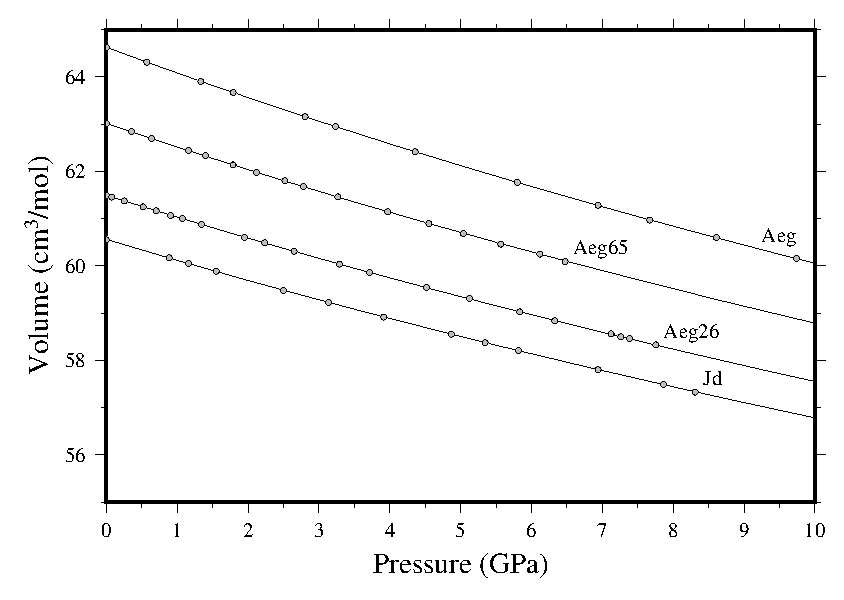
\includegraphics[width=0.8\textwidth]{figures/jadeite_aegirine_P_V}
  \caption{Pressure-volume data in the binary system jadeite-aegirine \citep{NBLBT2006}. Solid lines correspond to the volumes predicted by the model proposed in this study.}
  \label{fig:PV_jadeite_aegirine}
\end{figure}

\begin{table}[ht!]
\centering
\caption{Jadeite-Aegirine mixing parameters to fit the room temperature data of \cite{NBLBT2006}. The $K'_0$ for the intermediate compound is fixed to the value given by the heuristic proposed in the text. $K''_0 = -K'_0/K_0$.}
\label{tab:jd_aeg}
\begin{tabular}{lllll}
                   & jadeite              & aegirine             & jd$_{50}$ae$_{50}$             & ae$_{50}$jd$_{50}$             \\
$V_0$ (cm$^3$/mol) & 60.5640 $\pm$ 0.0001 & 64.6261 $\pm$ 0.0004 & 62.3641 $\pm$ 0.0005 & 62.4522 $\pm$ 0.0005 \\
$K_0$ (GPa)        & 133.5 $\pm$ 0.2      & 116.0 $\pm$ 0.2      & 124.8 $\pm$ 0.5      & 126.7 $\pm$ 0.4      \\
$K'_0$             & 4.6 [fixed]                 & 4.4 [fixed]                 & 4.4785 [heuristic]              & 4.4785  [fixed]           
\end{tabular}
\end{table}

Using the derived properties of the solid solution, we can fit the excess volume as a function of pressure (Figure \ref{fig:excess_volume_jadeite_aegirine}). The decay of excess volume as a function of pressure is in excellent agreement with the prediction that excess volumes decay to zero at extreme pressures. For the 50:50 intermediate, our excess bulk moduli and volumes indicate that $\xi \sim$ 11 (Equation \ref{K_T_heuristic}).

\begin{figure}[ht!]
  \centering
  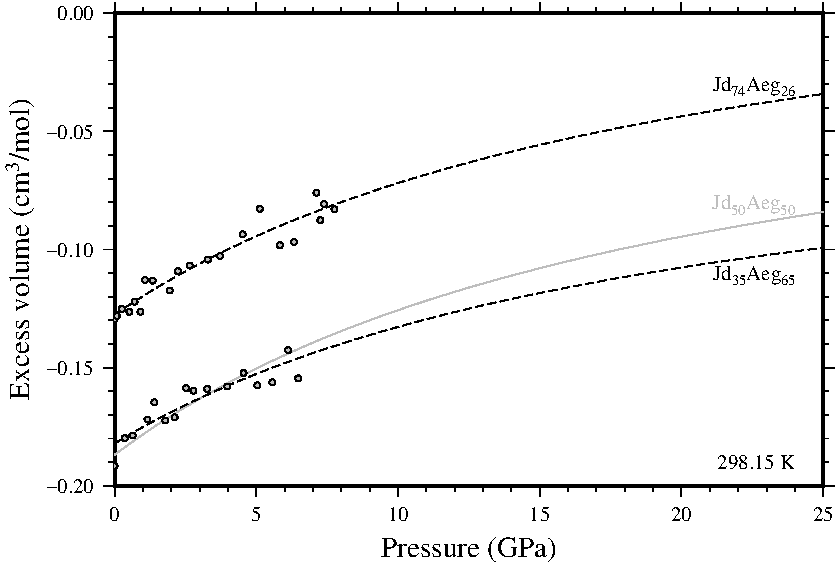
\includegraphics[width=0.8\textwidth]{figures/jadeite_aegirine_Vex}
  \caption{Excess volume for jadeite-aegirine pyroxenes \citep{NBLBT2006}. Solid lines correspond to the modelled excess volumes.}
  \label{fig:excess_volume_jadeite_aegirine}
\end{figure}

\subsection{Garnet}
Our first example dealt with a solid solution which has small excess volumes, but some phases exhibit significantly larger excesses. One example is the garnet system. Of particular interest is the pyrope-grossular join. Grossular is a major secondary component of many natural pyropic garnets. The size mismatch between the small magnesium cation and the large calcium cation on the dodecahedral site results in a large positive excess volume \citep{NCK1977, BG1997, GCT1996}. Recently, it has been suggested that the excess volumes of mixing are $\sim$1 cm$^3$/mol, 2--3 times larger than previously considered, and associated with very large negative excess bulk moduli \citep{DCW2015}. It is proposed that the differences are due to a hydrogrossular component in the crystals synthesised in piston cylinder apparatus in earlier studies, which becomes unstable at high pressures. Such a large variation in bulk modulus would have a major impact on seismic velocities and excess properties at high pressure. Since garnets remain stable to the uppermost lower mantle, a careful analysis of these effects is warranted.

Here, we create four models to describe the room temperature equations of state for the pyrope-grossular system using the pyrope and grossular endmembers from \cite{HP2011}. Two models are presented for the data of \citep{DCW2015}, to describe the reported behaviour close to the center and at the edges of the solid solution. The third model is the constant volume subregular Margules model of \cite{GCT1996}. A fourth model has the same excess volume as \cite{GCT1996}, but a negative excess bulk modulus which allows the excess volume to decay to zero at high pressures ($\xi=6$). The standard state bulk moduli are shown in Figure \ref{fig:K_T_pyrope_grossular}.


\begin{figure}[ht!]
  \centering
  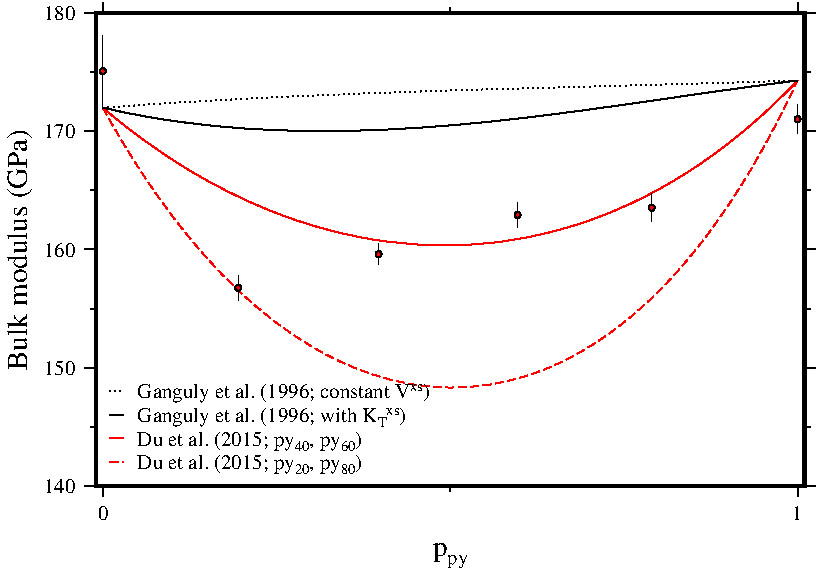
\includegraphics[width=0.8\textwidth]{figures/pyrope_grossular_K_0}
  \caption{Bulk moduli in the pyrope-grossular binary. Data points are those reported by \cite{DCW2015}. The four models correspond to those discussed in the main text.}
  \label{fig:K_T_pyrope_grossular}
\end{figure}

It is immediately obvious that the bulk moduli calculated from the \cite{DCW2015} study exhibit very large deviations from a linear trend. The symmetric curve derived from the two compounds in the middle of the binary yields $\xi=10$, a value which is not unreasonable, and results in a change in sign of the volume excess at 20--25 GPa. In contrast, the trend derived from the compounds with 20\% and 80\% pyrope content yields $\xi=52$. This extreme value leads to negative excess volumes at 5--6 GPa, which does not seem to be very likely. To avoid this, $K'_T$ must be increased to $>$20, which is also extremely unlikely.

The trend calculated from the terms in \cite{GCT1996} has a small positive excess bulk modulus, which is always the case where $\mathcal{V}^{xs}$ is held fixed. For the reasons outlined in the introduction, this is probably unlikely. The final model, constructed using the heuristics described in the previous section yields an excess bulk modulus on the order of 2--3 GPa.

These models are now used to illustrate the effect of different excess volume models on seismic wave velocities. P-wave, S-wave and bulk sound velocities are functions of isentropic bulk and shear moduli and density:
\begin{eqnarray}
V_P = \sqrt \frac{K_S + \frac{4}{3} G }{\rho} \\
V_S = \sqrt \frac{G}{\rho} \\
V_\Phi = \sqrt \frac{K_S}{\rho}
\end{eqnarray}
Thermodynamic solution models say nothing about shear moduli, so we restrict our discussion to the bulk sound velocity. Figure \ref{fig:bulk_sound_garnet} shows the bulk sound velocity at ambient temperature for the four solid solution models in the text. The models of \cite{DCW2015} result in large depressions of bulk sound velocity. The model constructed from the py$_{40}$ and py$_{60}$ samples results in a 4\% depression relative to the constant $\mathcal{V}^{xs}$ case throughout the upper mantle pressure range. In contrast, the model based on the excess volume model proposed in \cite{GCT1996} predicts a 1\% decrease in bulk sound speed. 

\begin{figure}[ht!]
  \centering
  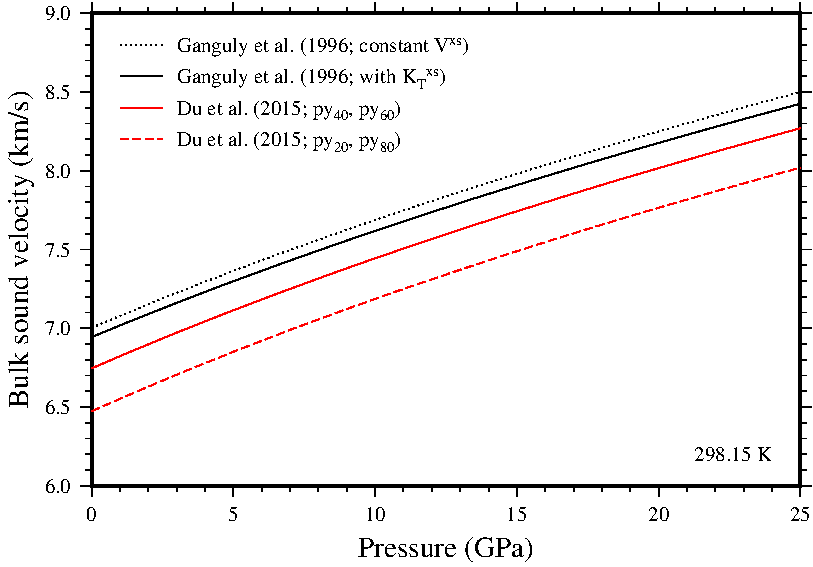
\includegraphics[width=0.8\textwidth]{figures/pyrope_grossular_bulk_sound_velocities}
  \caption{Bulk sound velocities of py$_{50}$gr$_{50}$ at room temperature according to the models described in the text and in Figure \ref{fig:K_T_pyrope_grossular}.}
  \label{fig:bulk_sound_garnet}
\end{figure}

It is not yet clear whether natural garnets have P-V-T equations of state similar to those suggested by \cite{DCW2015}, or similar to those in previous studies \citep{NCK1977, BG1997, GCT1996}. If a hydrogrossular component is indeed the cause for low excess volumes in piston cylinder-synthesised garnets, then garnets in the mantle are likely to have relatively high volume excesses and low bulk moduli. In this case, constant V$^{xs}$ models are clearly inappropriate both for calculations of mantle phase relations and seismic velocities. Even in the case of the model derived from \cite{GCT1996}, the difference in free energy compared with the constant V$^{xs}$ model is on the order of kilojoules at the bottom of the mantle transition zone. 

The heuristics suggested here place constraints on seismic properties which are significantly more strict than typical uncertainties on bulk moduli derived from ultrasonic interferometry, Brillouin scattering or static compression. For example, along the pyrope-majorite join, excess volumes are small (0.1 cm$^3$/mol) \citep{HSSR1997}. With the assumption that excess volumes decrease to zero with increasing pressure, the excess bulk modulus is constrained to be $\sim$-0.6 GPa. In comparison, the range in bulk modulus estimates anywhere along the pyrope-majorite join is about 10 GPa \citep[see, for example][]{HDLWB2010}. So far, high pressure elasticity studies have mostly been focussed on binary joins with small excess volumes at ambient pressure \citep{FXMLX2015, HC2014}. That they should exhibit small excess bulk moduli is in excellent agreement with the heuristics proposed here, but a far more rigorous test would be to investigate systems with large volume excesses.

\subsection{Metallic-ionic melt}
The thermodynamics and thermoelastics of ionic and metallic melts is fundamental to our understanding of core differentiation. During the formation of the terrestrial planets, it is thought that oligarchic growth led to a series of mixed silicate-metallic magma oceans, from which metallic melts separated before sinking as diapirs into the growing core \citep{Rubieetal2015}. Although these melts are predominantly composed of iron and nickel, several weight percent of light elements are required to explain the Earth's density deficit and low seismic velocities \citep{Poirier1994}. These light elements not only influence the melting point of the core (which directly informs us about the temperature of the inner core boundary), but also the style of crystallisation, and therefore the generation of a magnetic dynamo \citep{SSWL2007}. Since equilibration with a magma ocean governs the initial composition of the core, and seismology presents us with the most direct information on the present composition of the core, accurate thermodynamic modelling is vitally important to our understanding of the evolution and present chemical state of the Earth. It is well known that several iron-light element binaries are associated with large non-idealities \citep[e.g.][]{Frostetal2010}, so accurate modelling requires changes in excess properties in these systems to be taken into account.

Oxygen is a good example of a light element which exhibits a large degree of non-ideality. At pressures $<$25 GPa, the Fe-FeO solution exhibits significant non-ideality, with a large miscibility gap between ionic and metallic Fe-O liquids \citep{KS1995,TOT2007,Frostetal2010}. As pressure increases, this miscibility gap disappears, indicating a negative excess volume of mixing (Figure \ref{fig:Fe_O_solvus}).

\begin{figure}[ht!]
  \centering
  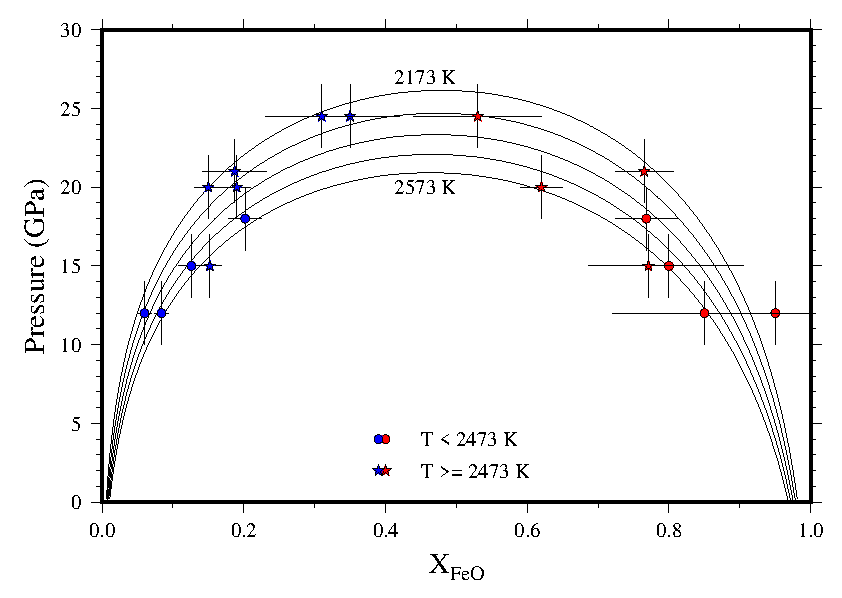
\includegraphics[width=0.8\textwidth]{figures/Fe_FeO_solvus}
  \caption{The Fe-FeO solvus as a function of pressure and temperature. Data points are taken from the studies of \cite{TOT2007} and \cite{Frostetal2010}. The model corresponds to the values proposed in Table \ref{tab:Fe_FeO}.}
  \label{fig:Fe_O_solvus}
\end{figure}

To constrain the properties of the Fe-FeO solid solution, the chemical potentials of Fe and FeO are estimated from the compositions of coexisting ionic and metallic melts at $<$25 GPa, and the pressure, temperature and compositions of eutectic liquid at $>$25 GPa \citep{SHCPW2008}. The latter constraints also require thermodynamic data for the eutectic phases (B1-structured FeO and FCC and HCP iron), which are calculated from room pressure data and constraints on the melting curves \citep{SHCPW2008, OTHOH2011, ADMLM2013, Kom2014}.  The Margules parameters estimated from this data are shown in Figure \ref{fig:Fe_O_interaction}. 

\begin{figure}[ht!]
  \centering
  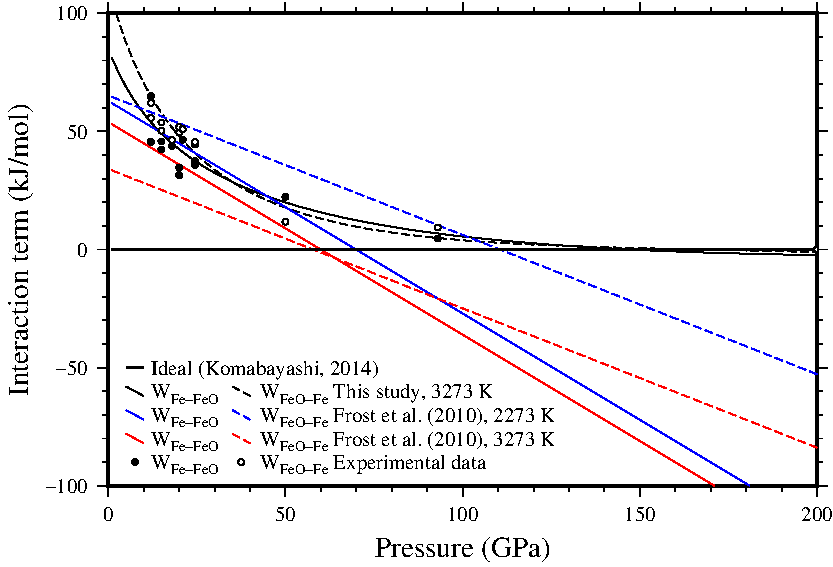
\includegraphics[width=0.8\textwidth]{figures/Fe_FeO_interaction_terms}
  \caption{Interaction terms in Fe-FeO melt as a function of pressure. Experimental data comes from solvus constraints at $<$25 GPa \citep{TOT2007,Frostetal2010}, and the composition and temperature of the eutectic at higher pressures \citep{SHCPW2008}.}
  \label{fig:Fe_O_interaction}
\end{figure}

The uncertainties on composition and temperature of the eutectic are rather large, so these data are supplemented by the requirement that excess volumes become zero at very high pressure. The parameters used to create the fits in Figures \ref{fig:Fe_O_interaction} and \ref{fig:Fe_O_melting} are given in Table \ref{tab:Fe_FeO}. It is assumed that excess entropy and thermal expansion are negligible. The majority of the $<$25 GPa data was collected within a $\sim$200 K temperature range, and is associated with similar temperature uncertainties, which introduces very large uncertainties in excess entropies. Add to that the possibility of phase separation during quench and the large uncertainty in coexisting ionic/metallic melt compositions, there is no clear evidence for the large temperature dependence proposed by \cite{Frostetal2010}, although they do slightly improve the fit to the data (mostly by increasing the pressure at which the solvus closes at high temperature).

\begin{figure}[ht!]
  \centering
  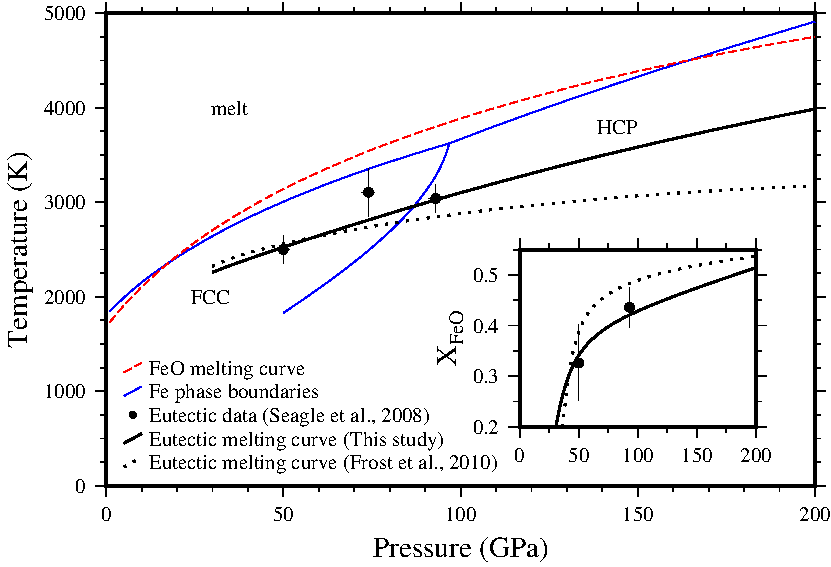
\includegraphics[width=0.8\textwidth]{figures/Fe_FeO_T_X_eutectic}
  \caption{Melting temperature in the Fe-O system as a function of pressure. Inset: eutectic composition in the Fe-O system. Data points are from \cite{SHCPW2008}. The model of \cite{Frostetal2010} employs constant volume and entropy terms derives from data obtained at $<$25 GPa, and deviates significantly from experimental constraints at pressures corresponding to the Earth's core.}
  \label{fig:Fe_O_melting}
\end{figure}

\begin{table}[ht!]
\centering
\caption{Excess Fe-FeO mixing parameters to fit the data in Figures \ref{fig:Fe_O_interaction} and \ref{fig:Fe_O_melting} at a reference temperature of 1809 K and pressure of 50 GPa.}
\label{tab:Fe_FeO}
\begin{tabular}{lll}
  Property        & Fe$_{50}$FeO$_{50}$  & FeO$_{50}$Fe$_{50}$ \\
  $H^{xs}$ (J/mol) &  5000 $\pm$ 400 & 4400 $\pm$ 400  \\
  $S^{xs}$ (J/K/mol)  & 0 [fixed] & 0 [fixed] \\
  $V^{xs}$ (cm$^3$/mol)   & -0.117 $\pm$ 0.009 &  -0.138 $\pm$ 0.009 \\
  $K^{xs}$  (GPa)  & 28 $\pm$ 5 & 45 $\pm$ 5  \\
  $K'^{xs}$   & -0.07 $\pm$ 0.12 & -0.37 $\pm$ 0.12  \\
  $a^{xs}$   & 0 [fixed] & 0 [fixed]  
\end{tabular}
\end{table}


The constant negative volume excesses in the model of \cite{Frostetal2010} produce reasonable eutectic melting temperatures up to $\sim$ 50 GPa. Beyond this point, the increasing pressure stabilisation of the solution results in large deviations from the slope of the melting curve (Figure \ref{fig:Fe_O_melting}). This effect becomes very large at inner core boundary pressures (330 GPa), where solid Fe and FeO are stable to at least $\sim$4200 K \citep{OTHOH2011}. In contrast, the melting point derived from the parameters of \cite{Frostetal2010} reaches a maximum at 3225 K and 275 GPa. The best fit excess bulk moduli in Table \ref{tab:Fe_FeO} are large, even at the reference pressure of 50 GPa. Such values will have a significant effect on seismic velocities, especially at the pressures corresponding to the cores of small planetary bodies.


\section{Discussion}
% Intro
The use of intermediate compounds to describe excess properties within the framework of simple solution models lends the flexibility required to create single thermoelastodynamic models covering very large \emph{P-T} ranges. In this study, the high pressure properties of pyroxenes, garnets and melts are used to illustrate the development of such models, and their ability to accurately reproduce observed variations in pressure, temperature or compositional derivatives of the Gibbs free energy, such as bulk modulus and chemical potentials. Without these, it would be impossible to accurately model phase relations at extreme conditions, or seismic velocities.

This study does not discuss the behaviour of the shear modulus across solid solutions. Thermodynamic databases are now starting to include shear moduli and their change with pressure and temperature \citep{SLB2011}, so constraining these changes across solid solutions should also be a key priority for experimental and ab-initio studies. Using intermediate compounds to describe the change in shear modulus across a solid solution should work well, especially in silicate systems, where excess shear moduli may be of similar magnitude to excess bulk moduli, and also decrease with increasing pressure \citep[e.g][]{LEDD2014}.

% Heuristics
The heuristics suggested in this study agree with the available data on the three example systems, but remain heuristics only. It would be particularly interesting to investigate the change in excess volumes with temperature and pressure for other systems in which excess properties are large, and interpret these in terms of crystal or melt structures. Conversely, the behaviour of systems with small excesses at room temperature and pressure should also be investigated. Current evidence suggests that small volume excesses at low pressure remain small under different conditions \citep{FXMLX2015, HC2014}, but this may not be true for all solutions.

% Other planets
In the case of ionic and metallic melts, excess volumes can be extremely large at low pressure. The large excess elastic moduli accompanying these excess volumes will have a large effect on seismic velocities, especially in the cores of relatively small bodies such as Mars or the Moon. As pressures increase, excess volumes are much reduced, which has a similarly profound effect on thermodynamic properties \citep{Frostetal2010, DKS2013}. Accurate characterisation of excess properties of melt solutions, and indeed of solutions in general, will become increasingly important for our interpretation of seismic anomalies, modelling of phase relations, and our understanding of planetary evolution. 


\section{Acknowledgments}
RM is funded by the Advanced ERC Grant awarded to the ``ACCRETE'' project (Contract number 290568). He would like to thank Dave Rubie, Dan Frost and Christopher Beyer for useful discussions.

Figures were created using the Generic Mapping Tools \citep{GMT}.
\clearpage
\section*{References}

\bibliography{references_xs}

\end{document}
